\subsubsection{UI Design}

Building on the navigation flow and functional description presented in the previous sections, this section provides a visual overview of the application's user interface. The following screenshots illustrate the main screens, their layout, and the interface states relevant to the user workflow. Additional interface variations and supplementary views are included in Appendix \ref{appendix:user_interface_gallery} for completeness.

\textbf{LoginPage View}

Figure \ref{fig:login-page-view} displays the UI corresponding to the application's secure access portal. This page is shown when the user accesses the application for the first time or when the session has expired.

\begin{figure}[H]
    \centering
    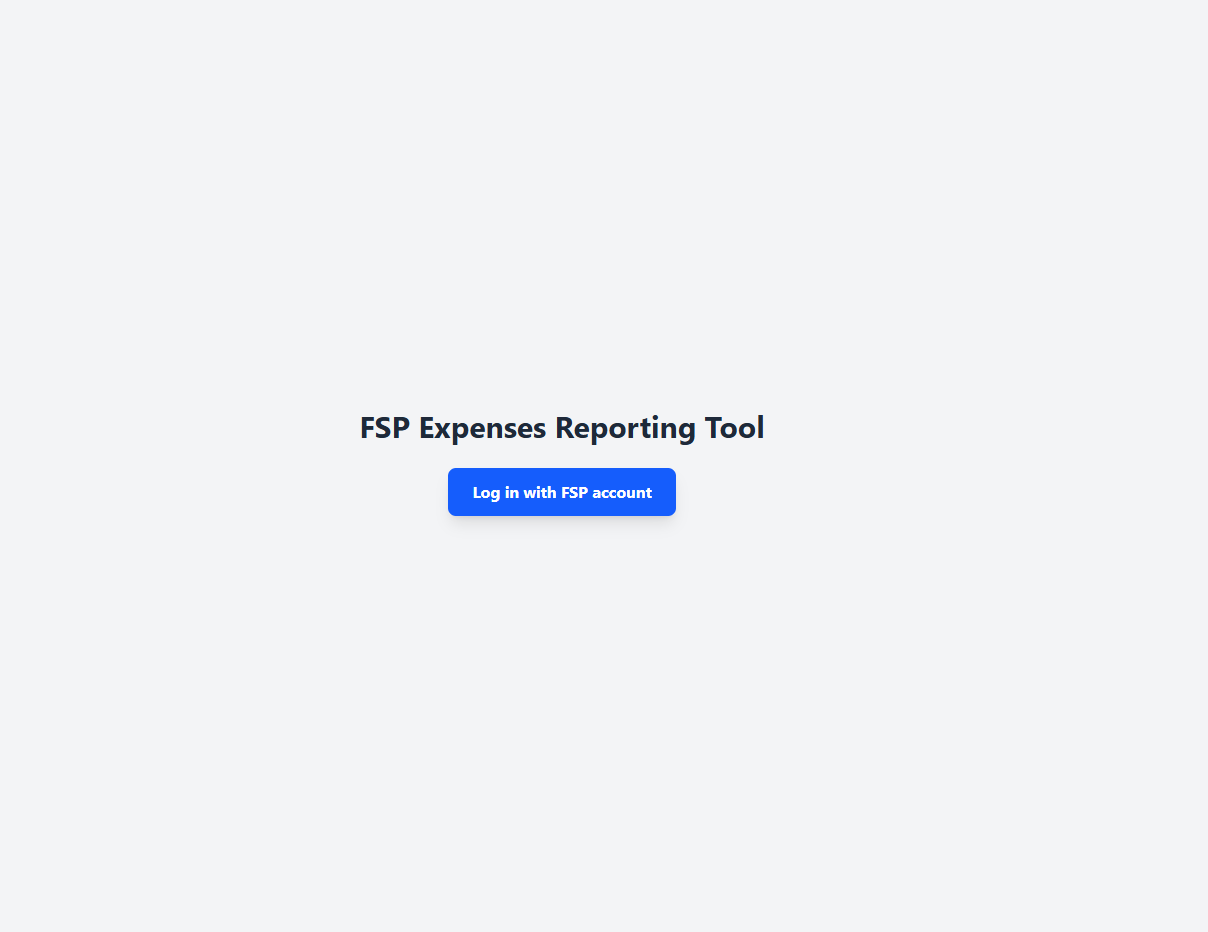
\includegraphics[width=0.8\textwidth]{Images/UIDesign/LoginPage.png}
    \caption[LoginPage user interface view]
    {LoginPage user interface view. [Own creation]}
    \label{fig:login-page-view}
\end{figure}

 
\textbf{ExpensesPage View}

This is the ExpensesPage view, where users can perform all expense-related tasks. In the UI shown in Figure \ref{fig:expenses-page-view}, users can upload multiple receipt files or images for processing and view the real-time AI processing status of an expense. Users can also search or filter uploaded expenses, as shown in Figure \ref{fig:expenses-search-filter-view}. Another feature of this page is the ability to attach expenses with a ``Reviewed'' status to a new or existing report. This last feature is illustrated in Figure \ref{fig:expenses-page-assign-report-view-appendix} from Appendix \ref{appendix:user_interface_gallery}.

\begin{figure}[H] 
    \centering
    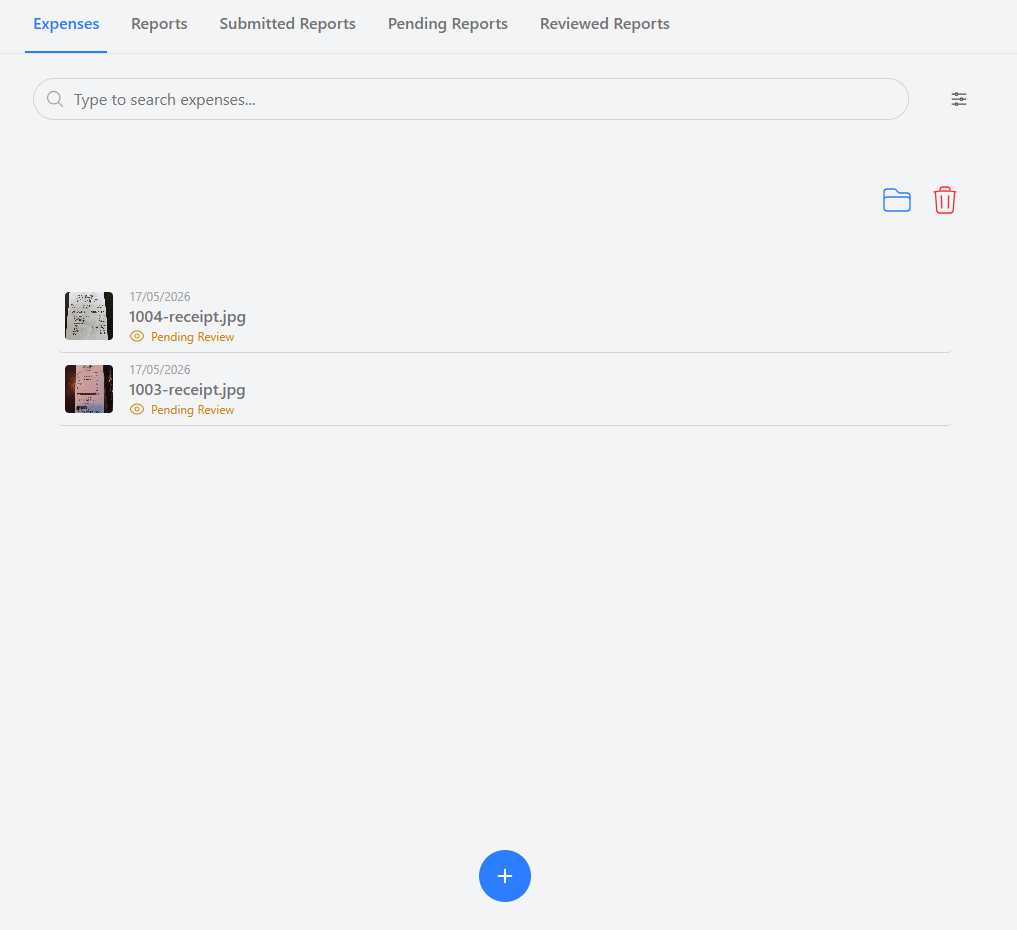
\includegraphics[width=0.65\textwidth]{Images/UIDesign/ExpensesPage.png}
    \caption[ExpensesPage user interface view]
    {ExpensesPage user interface view. [Own creation]}
    \label{fig:expenses-page-view}
\end{figure}


\begin{figure}[H] 
    \centering
    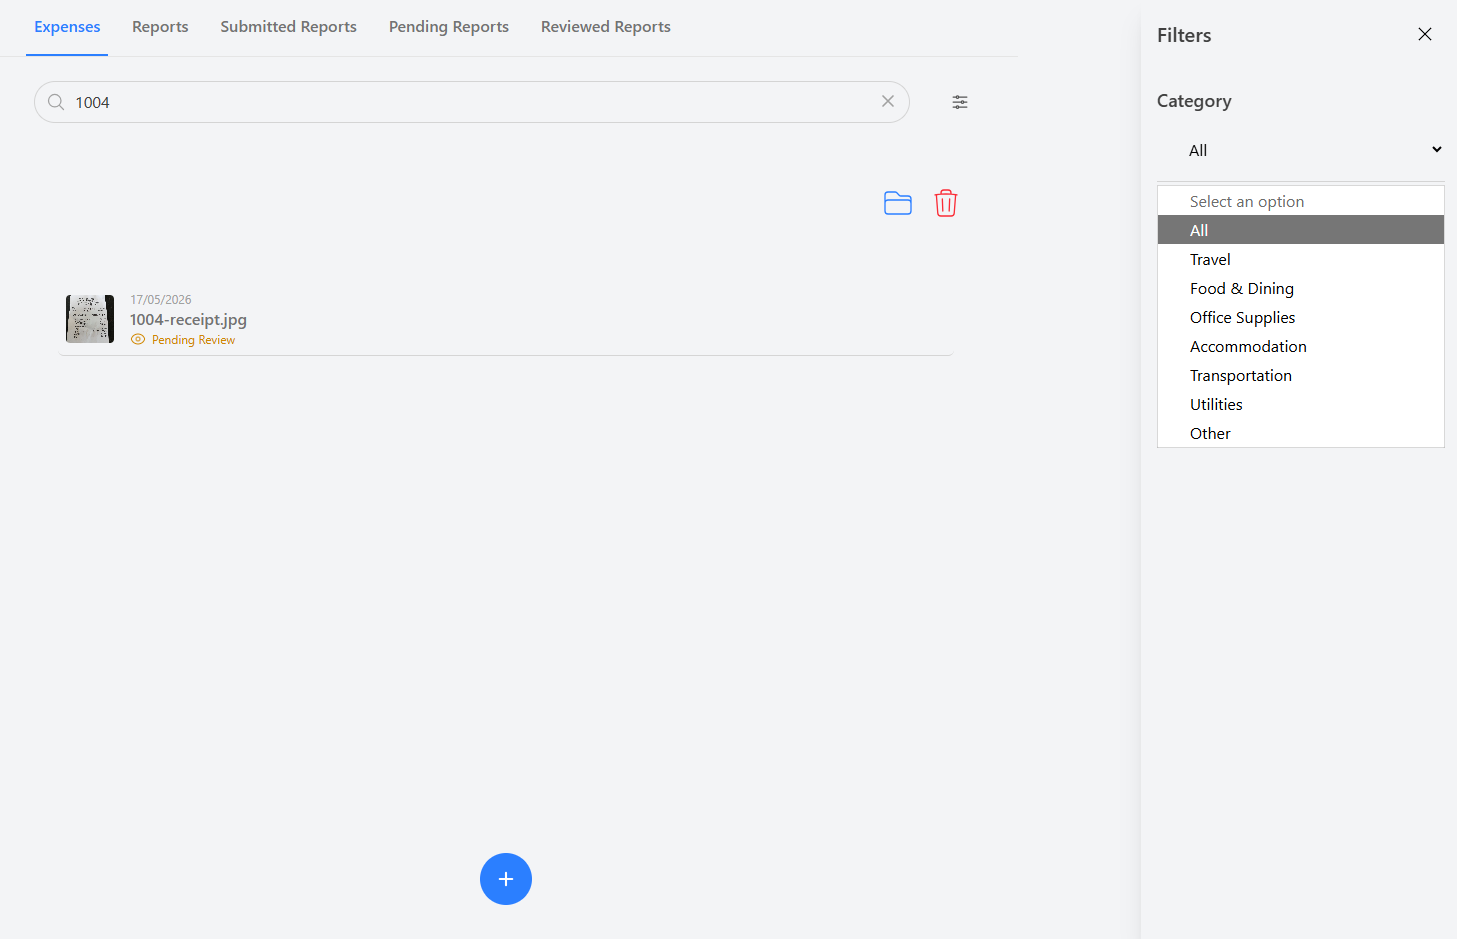
\includegraphics[width=0.75\textwidth]{Images/UIDesign/ExpenseSearchAndFilter.png}
    \caption[ExpensesPage user interface view for filtering by category and name]
    {ExpensesPage user interface view for filtering by category and name. [Own creation]}
    \label{fig:expenses-search-filter-view}
\end{figure}


\textbf{ReportsPage View}

In the ReportsPage view in Figure \ref{fig:reports-page-view}, users can view all reports they have created that are pending submission. The subsequent Figure \ref{fig:create-report-from-reports-page-view} also illustrates the same page, which allows users to create new reports attaching expenses with a ``Reviewed'' status and delete existing reports.

\begin{figure}[H] 
    \centering
    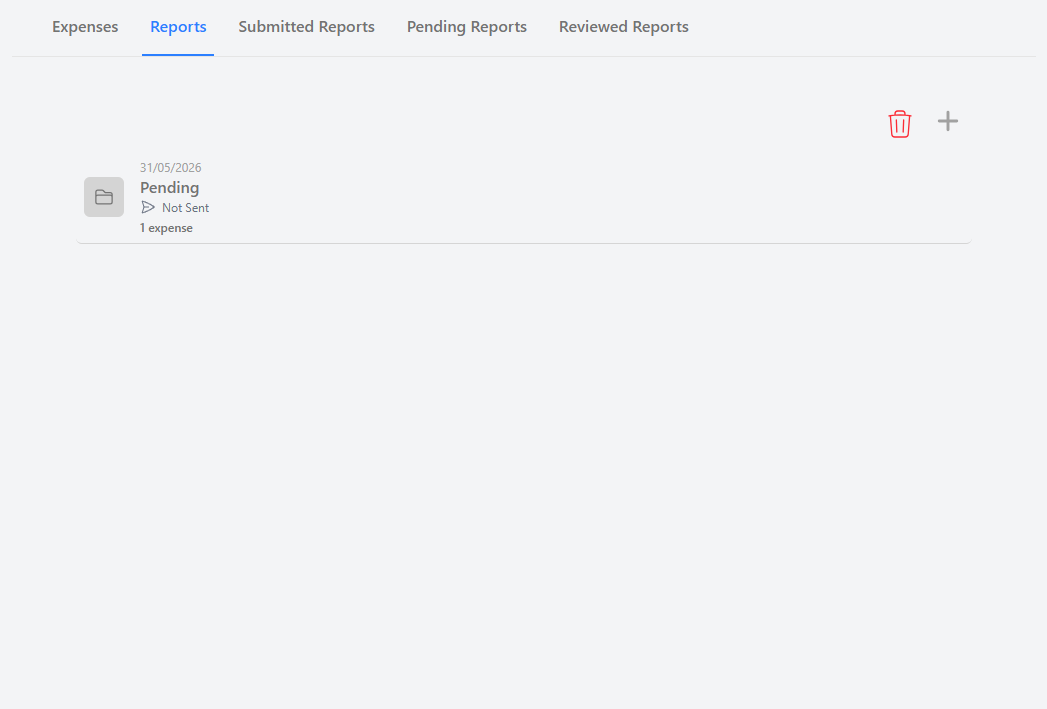
\includegraphics[width=0.75\textwidth]{Images/UIDesign/ReportsPage.png}
    \caption[ReportsPage user interface view]
    {ReportsPage user interface view. [Own creation]}
    \label{fig:reports-page-view}
\end{figure}

\begin{figure}[H] 
    \centering
    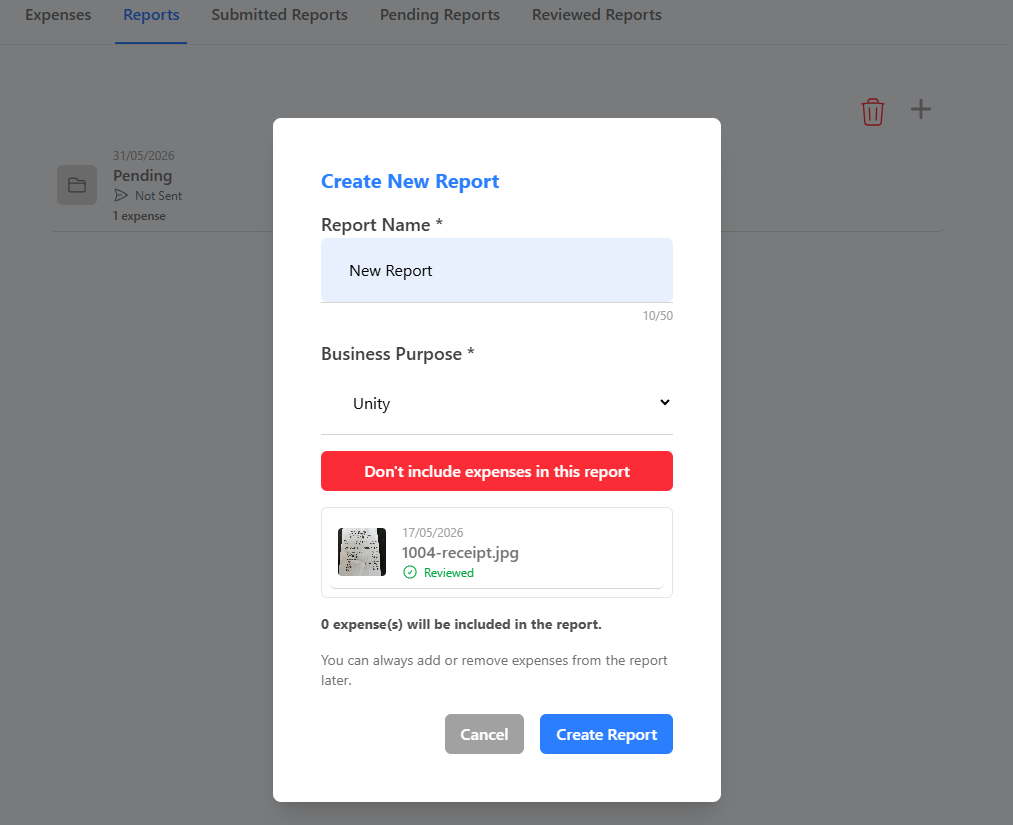
\includegraphics[width=0.75\textwidth]{Images/UIDesign/CreateReportFromReportsPage.png}
    \caption[ReportsPage user interface view for creating a new report]
    {ReportsPage user interface view for creating a new report. [Own creation]}
    \label{fig:create-report-from-reports-page-view}
\end{figure}


\textbf{ExpenseInfoPage View}

If an uploaded expense is successfully processed by the AI, the user can enter the corresponding ExpenseInfoPage view (Figure \ref{fig:expense-info-page-view}) to review and correct the AI-extracted information. If the AI extraction fails, the user can also enter the same page to manually enter the expense information.

\begin{figure}[H] 
    \centering
    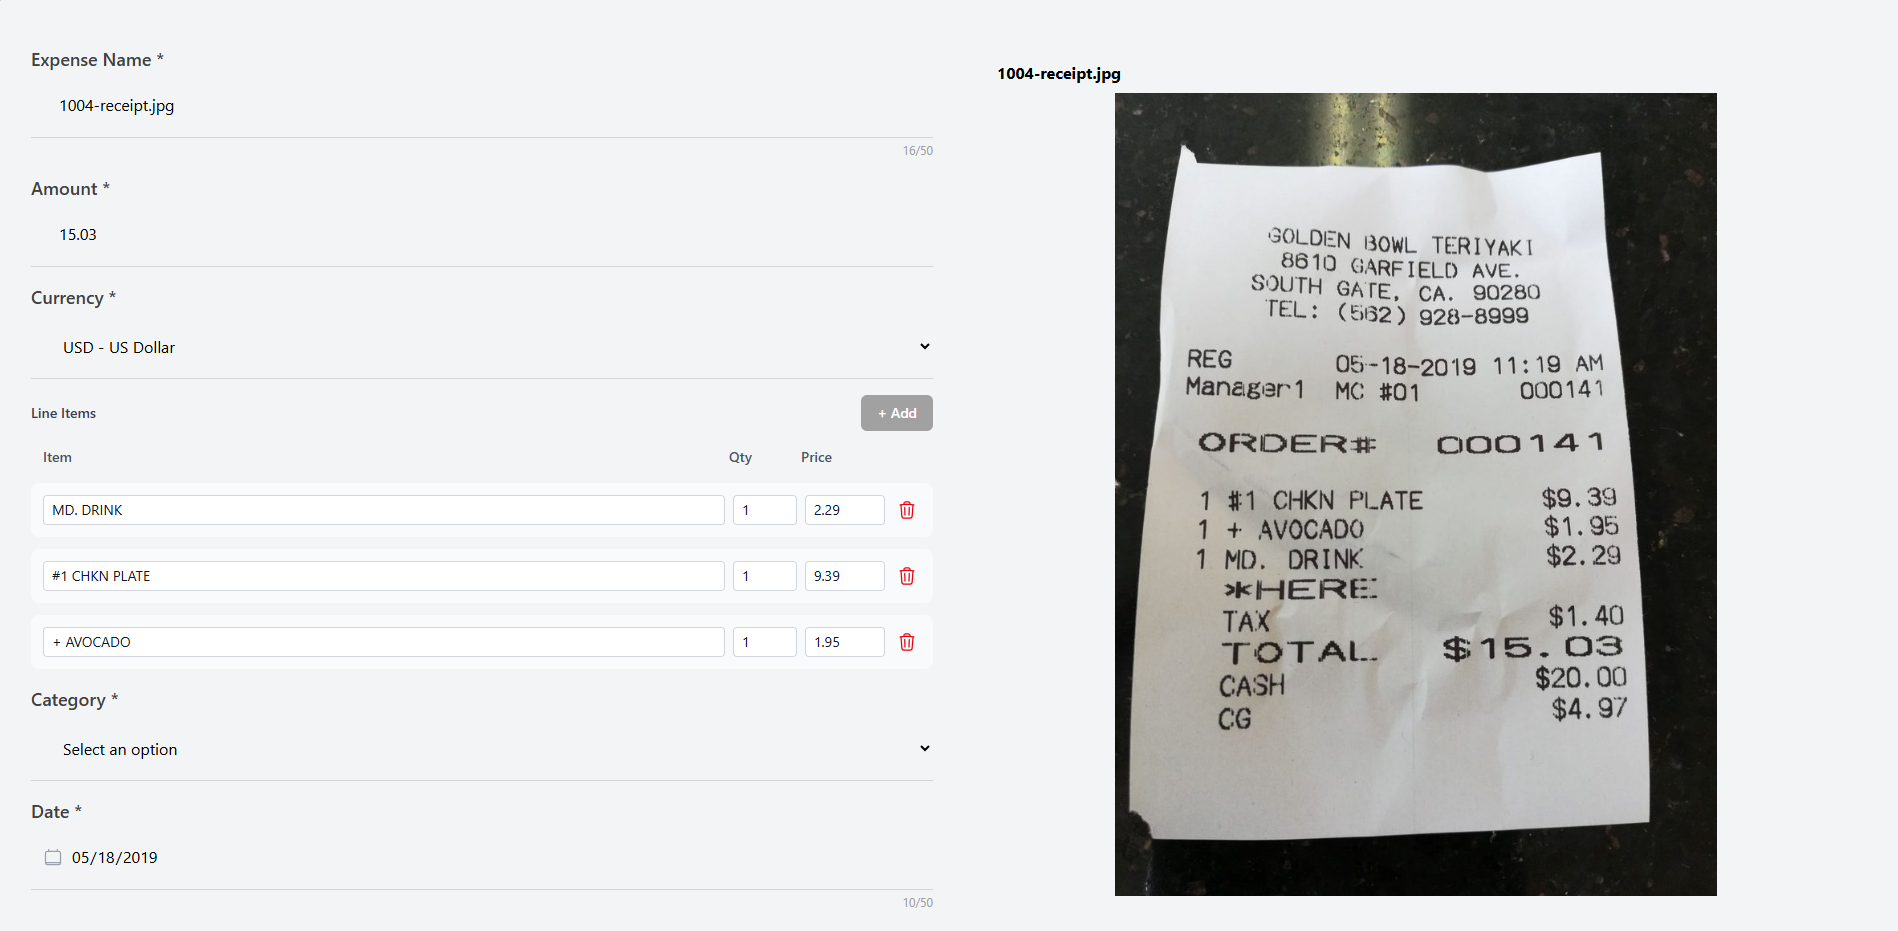
\includegraphics[width=\textwidth]{Images/UIDesign/ExpenseInfoPage.png}
    \caption[ExpenseInfoPage user interface view]
    {ExpenseInfoPage user interface view. [Own creation]}
    \label{fig:expense-info-page-view}
\end{figure}

\textbf{ReportInfoPage View}

The last UI is the ReportInfoPage view displayed in Figure \ref{fig:report-info-page-view}. Here, the user can review and modify the detailed information of each expense. On the right side, the user can attach or detach expenses from the current report and navigate to the attached expenses' ExpenseInfoPage views as well.
\begin{figure}[H] 
    \centering
    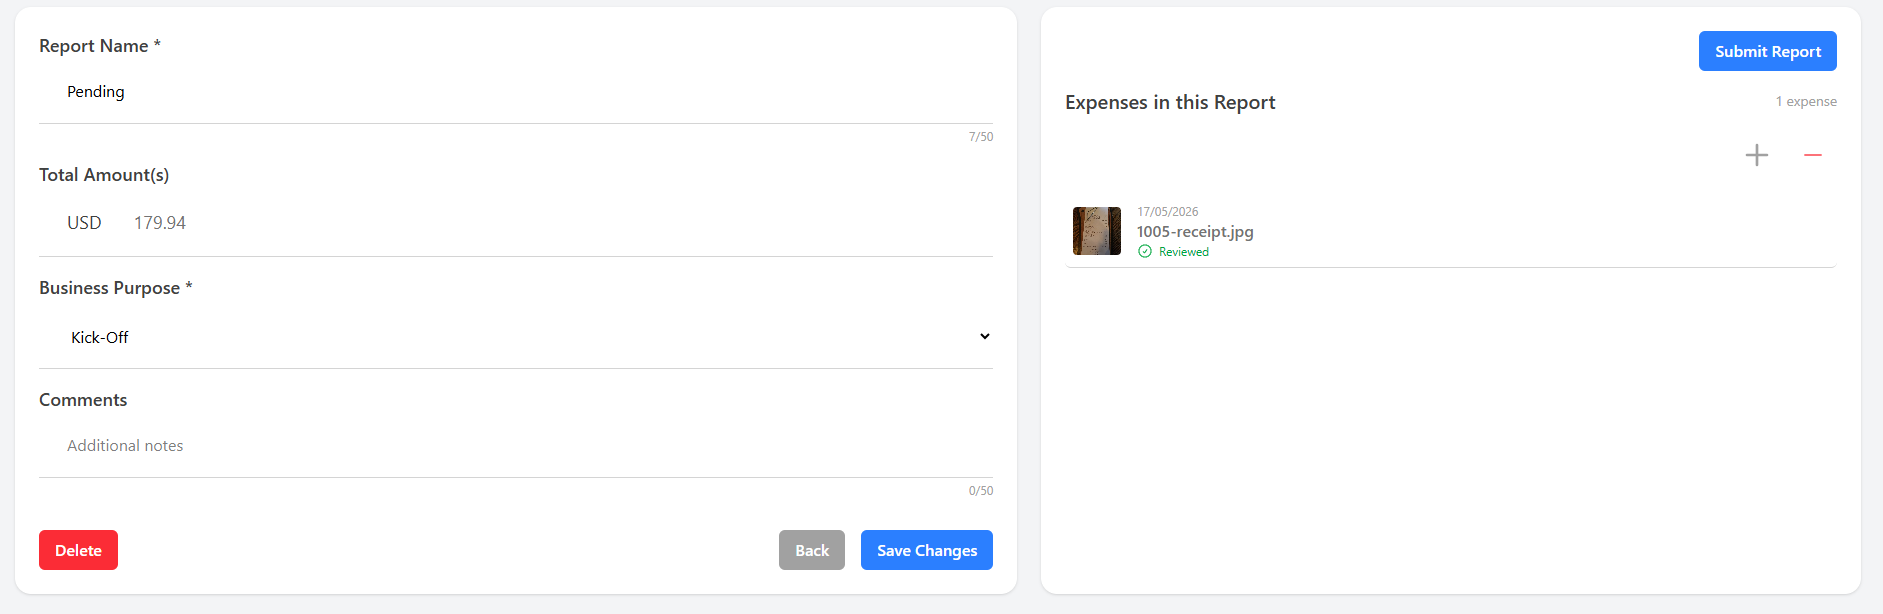
\includegraphics[width=\textwidth]{Images/UIDesign/ReportInfoPage.png}
    \caption[ReportInfoPage editable user interface view]
    {ReportInfoPage editable user interface view. [Own creation]}
    \label{fig:report-info-page-view}
\end{figure}
